\documentclass{amsart}
\usepackage[T1]{fontenc}
%\usepackage{mathpazo}
%\usepackage[margin=1in]{geometry}
\usepackage[inline]{enumitem}
%\usepackage{rotating}
%\usepackage{color}
%\usepackage{tabu}
%\usepackage{parskip}
\usepackage{graphicx}
\usepackage{caption}
\usepackage{subcaption}
\usepackage{multicol}
\usepackage{booktabs}
\usepackage{hyperref}
\usepackage{amsmath}
\usepackage{amssymb}
\usepackage{amsthm}
\usepackage{calc}
\usepackage{xfrac}
\usepackage{mathtools}
\usepackage{cancel}
\usepackage{framed}
\usepackage{nth}
\usepackage{tikz}
\usetikzlibrary{calc,decorations.markings}
%\usepackage{xcolor-solarized}
%\usepackage{minted}
%\usepackage{MnSymbol}
%\usepackage[libertine]{newtxmath}
%\newcommand*\circled[1]{\tikz[baseline= (char.base)]{
    %\node[shape=circle,draw,inner sep=2pt] (char) {#1};}}
%\usepackage{xypic}
%\usepackage[tightpage]{preview} % display
% Math operators
\DeclareMathOperator{\Z}{\mathbb{Z}}
\DeclareMathOperator{\Q}{\mathbb{Q}}
\DeclareMathOperator{\N}{\mathbb{N}}
\DeclareMathOperator{\R}{\mathbb{R}}
\DeclareMathOperator{\C}{\mathbb{C}}
\DeclareMathOperator{\F}{\mathbb{F}}
\DeclareMathOperator{\sge}{\mathsf{e}}
\DeclareMathOperator{\sgm}{\mathsf{m}}
\DeclareMathOperator{\sgG}{\mathsf{G}}
\DeclareMathOperator{\sgg}{\mathsf{g}}
\DeclareMathOperator{\sgF}{\mathsf{F}}
\DeclareMathOperator{\sgt}{\mathsf{t}}
\DeclareMathOperator{\sgL}{\mathsf{L}}
\DeclareMathOperator{\sgZ}{\mathsf{Z}}
\DeclareMathOperator{\sgAp}{Ap}
\DeclareMathOperator{\sgPF}{PF}
\DeclareMathOperator{\sgconv}{conv}
\DeclareMathOperator{\sgsupp}{supp}
\DeclareMathOperator{\calC}{\mathcal{C}}
\DeclareMathOperator{\calF}{\mathcal{F}}
\DeclareMathOperator{\calO}{\mathcal{O}}
\DeclareMathOperator{\Grho}{\prescript{}{\rho}G}
% Theorem environments
\theoremstyle{plain}
\newtheorem{thm}{Theorem}
\newtheorem*{thm*}{Theorem}
\newtheorem{lemma}{Lemma}
\newtheorem*{lemma*}{Lemma}
\newtheorem*{claim}{Claim}
\newtheorem*{cor}{Corollary}
\newtheorem*{prop}{Proposition}
\newtheorem*{conj}{Conjecture}
\theoremstyle{remark}
\newtheorem*{example*}{Example}
\theoremstyle{definition}
\newtheorem*{definition*}{Definition}
% Special theorem displays
\newenvironment{example}%
	{\begin{leftbar}\begin{example*}
}{%
	\end{example*}\end{leftbar}
}
\newenvironment{definition}%
	{\begin{leftbar}\begin{definition*}
}{%
	\end{definition*}\end{leftbar}
}
% Paired math operators
\DeclarePairedDelimiter{\ceil}{\lceil}{\rceil}
\DeclarePairedDelimiter{\floor}{\lfloor}{\rfloor}
% Math helper functions
\newcommand{\congr}[2]{{[#1]}_{#2}}
\newcommand{\set}[1]{\{#1\}}
\newcommand{\genset}[1]{{\langle{}#1\rangle{}}}
\newcommand{\abs}[1]{\lvert{}#1\rvert{}}
\newcommand{\norm}[1]{\lVert{}#1\rVert{}}
\newcommand{\bmx}[1]{\begin{bmatrix}#1\end{bmatrix}}
\newcommand{\pmx}[1]{\begin{pmatrix}#1\end{pmatrix}}
  \newcommand{\sbmx}[1]{{\left[\begin{smallmatrix}#1\end{smallmatrix}\right]}}
\newcommand{\smallxymatrix}[2]{\xymatrix@C-=#1in@R-=#1in{#2}}
\renewcommand\labelitemi{\small$\bullet$}
%
%\makeatletter
\tikzset{%
  gdot/.style={draw,shape=circle,fill=black,inner sep=1},
  ddot/.style={draw,shape=circle,fill=white,inner sep=1},
  dedge/.style={draw=black!40},
  midarrow/.style={postaction={decorate},decoration={markings,mark=at position 0.5 with {\arrow{>}}}}
}
%\makeatother
\begin{document}
%
%
%

\section*{Prompt:}

\noindent
\begin{quote}
  (13) \emph{Flow polytopes.}
  A \emph{directed graph} is a collection of dots (called \emph{vertices}) and
  arrow between them (called \emph{edges}). A \emph{flow} on a directed graph is a
  way to label each edge of $G$ by an element of $\Z$ (or $\Z_n$) so that at each
  vertex $v$, the sum of the edges entering $v$ equals the sum of the edges
  leaving $v$ (i.e.\ the in \emph{flow} at each vertex equals the \emph{out
  flow}). The flows on a given directed graph can be counted using a certain
  family of polytopes, whose integer points each coincide with a flow on $G$.
  \\[1em]
  \noindent
  Source:
  \emph{Combinatorial reciprocity theorems} (M. Beck, R. Sanyal), Chapters 1 and 7.
\end{quote}

\hrulefill

Graphs are a major area of concern in mathematics, having an entire field to
study dedicated to them. Many different families of graphs exist, but for this
paper we'll concern ourselves with directed graphs and $\Z_n$-flows on these
graphs, all concepts which the first section introduces. The second section
is dedicated to a reciprocity expression for counting the number of possible
flows on directed graphs, and to developing some insight into it and its proof.

% ------------------------------------------------------------------------------
% 1.2
% ------------------------------------------------------------------------------


\section{Introduction to graphs and flows}

\subsection{Graphs}

A graph $G=(V,E)$ is a collection of $V$, a set of vertices, and $E$, a set of
edges between the vertices.
Now, a graph doesn't have to have any vertices, nor
does it have to to have any edges (except that if it has edges there must be
vertices to which those edges connect).
Also note that the nodes of a graph can be elements of some arbitrary
d-dimensional space, but for this report we'll only concern ourselves with
graphs in some two-dimensional space.
(Note that the word ``node'' is analogous to ``vertex'' and that this paper
will do plenty of haphazard switching between the two of them.)
\begin{definition}[Component, connected component]
  A \emph{connected component} (or simply a \emph{component}) of a graph $G$ is
  a subgraph (a subset of the vertices and edges of $G$) in which any two
  vertices are either directly connected via an edge or are connected to
  one-another via a \emph{path} (a series of vertices and edges). A single
  vertex with no connecting edges is in itself a connected component.
\end{definition}
Any graph then is the disjoint union of connected components.
For example Figure~\ref{fig:disjoint-union} can be called a single graph that is the disjoint
union of three distinct connected components.
\begin{figure}[ht]
  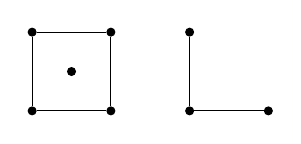
\begin{tikzpicture}[every node/.style=gdot]
    \path
      (.5,.5) node (a) {}
      (0,0) node (b) {} (1,0) node (c) {} (1,1) node (d) {} (0,1) node (e) {}
      (2,1) node (f) {} (2,0) node (g) {} (3,0) node (h) {};
    \draw (a);
    \draw (b) -- (c) -- (d) -- (e) -- (b);
    \draw (f) -- (g) -- (h);
  \end{tikzpicture}
  \caption[Disjoin union]{}
  \label{fig:disjoint-union}
\end{figure}
\begin{lemma*}
  A connected component of the graph $G$ is a maximal subgraph of $G$ in which
  any two nodes are connect by a path.
\end{lemma*}
\begin{lemma*}
  A graph $G$ is \emph{connected} if it has only one connected component.
\end{lemma*}
\begin{definition}[Bridge]
  A \emph{bridge} is a single edge which serves as a connection between two connected
  components which, if removed, would increase the number of connected
  components of the graph by one.
\end{definition}
For example, removing the bridge in Figure~\ref{fig:bridge} turns a single
connected component into two triangular connected components:
one complete graph into a graph with two complete subgraphs.
\begin{figure}[ht]
  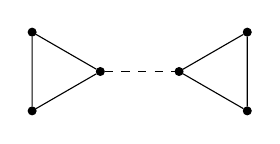
\begin{tikzpicture}[every node/.style=gdot]
    \path
      (-.5,.5) node (a) {} ($({-(1+sqrt(3))/2},0)$) node (b) {} ($({-(1+sqrt(3))/2},1)$) node (c) {}
      ( .5,.5) node (d) {} ($({ (1+sqrt(3))/2},0)$) node (e) {} ($({ (1+sqrt(3))/2},1)$) node (f) {};
    \draw (a) -- (b) -- (c) -- (a);
    \draw (d) -- (e) -- (f) -- (d);
    \draw[dashed] (a) -- (d);
  \end{tikzpicture}
  \hspace{1in}
  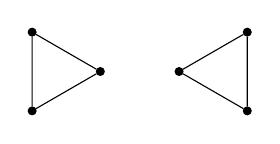
\begin{tikzpicture}[every node/.style=gdot]
    \path
      (-.5,.5) node (a) {} ($({-(1+sqrt(3))/2},0)$) node (b) {} ($({-(1+sqrt(3))/2},1)$) node (c) {}
      ( .5,.5) node (d) {} ($({ (1+sqrt(3))/2},0)$) node (e) {} ($({ (1+sqrt(3))/2},1)$) node (f) {};
    \draw (a) -- (b) -- (c) -- (a);
    \draw (d) -- (e) -- (f) -- (d);
  \end{tikzpicture}
  \caption[Bridges]{A graph with and without a bridge.}
  \label{fig:bridge}
\end{figure}

\subsection{Directed graphs}

So far we've only looked at \emph{unoriented} graphs, but
now we introduce a notion of direction, or orientation, to graphs.
\begin{definition}[Directed, oriented graph]
  A \emph{directed} or \emph{oriented graph} is a graph on which we
  define an \emph{orientation} via a subset $\rho$ of the edges $E$ of the
  graph. For each edge $e=v_i v_j\in E$ (connecting the vertices $v_i,v_j\in
  V$) with $i<j$ we direct:
  \[
    v_i\stackrel{e}{\leftarrow}v_j\text{ if }e\in\rho\text{, and }
    v_i\stackrel{e}{\rightarrow}v_j\text{ if }e\notin\rho.
  \]
\end{definition}
This definition may be confusing at first glance because $\rho$
may be missing some of the edges of $E$. What this definition attempts to succinctly
encapsulate is only the edges with their direction pointing from the vertex of higher
index to the vertex of lower index (which does certainly feel backwards),
with all the remaining edges not in $\rho$ directed in the opposite direction,
from lower to higher index.
Figure~\ref{fig:directed-graph} tries to illustrate this encapsulation for a graph
with five vertices and an orientation $\rho=\{14,23,24\}$.
\begin{figure}[ht]
  \begin{subfigure}[t]{0.3\textwidth}
    \centering
    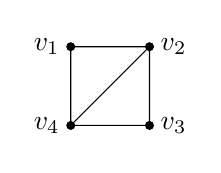
\begin{tikzpicture}[every node/.style=gdot]
      \path
        (0,1) node (v_1)[label=left:$v_1$]{}
        (1,1) node (v_2)[label=right:$v_2$]{}
        (1,0) node (v_3)[label=right:$v_3$]{}
        (0,0) node (v_4)[label=left:$v_4$]{};
      \draw (v_4) -- (v_3) -- (v_2) -- (v_1) -- (v_4) -- (v_2);
    \end{tikzpicture}
    \caption{The undirected graph.}
  \end{subfigure}
  %\hspace{1in}
  \begin{subfigure}[t]{0.3\textwidth}
    \centering
    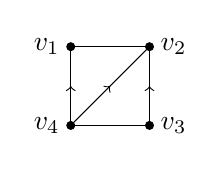
\begin{tikzpicture}[every node/.style=gdot]
      \path
        (0,1) node (v_1)[label=left:$v_1$]{}
        (1,1) node (v_2)[label=right:$v_2$]{}
        (1,0) node (v_3)[label=right:$v_3$]{}
        (0,0) node (v_4)[label=left:$v_4$]{};
      \draw[midarrow] (v_4) -- (v_1);
      \draw[midarrow] (v_4) -- (v_2);
      \draw[midarrow] (v_3) -- (v_2);
      \draw (v_3) -- (v_4);
      \draw (v_1) -- (v_2);
    \end{tikzpicture}
    \caption{$\rho$ edges marked.}
  \end{subfigure}
  \begin{subfigure}[t]{0.3\textwidth}
    \centering
    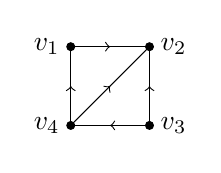
\begin{tikzpicture}[every node/.style={gdot}]
      \path
        (0,1) node (v_1)[label=left:$v_1$]{}
        (1,1) node (v_2)[label=right:$v_2$]{}
        (1,0) node (v_3)[label=right:$v_3$]{}
        (0,0) node (v_4)[label=left:$v_4$]{};
      \draw[midarrow] (v_4) -- (v_1);
      \draw[midarrow] (v_4) -- (v_2);
      \draw[midarrow] (v_3) -- (v_2);
      \draw[midarrow] (v_3) -- (v_4);
      \draw[midarrow] (v_1) -- (v_2);
    \end{tikzpicture}
    \caption{$E\setminus\rho$ edges marked.}
  \end{subfigure}
  \caption[A directed graph]{A directed graph.}
  \label{fig:directed-graph}
\end{figure}

As an aside, directed graphs are the subject of many algorithms in computer
science, often pertaining to finding optimal ways to traverse the paths of said
graphs. In some models each edge is considered to be of equal ``weight'' as any
other. That is if two edges originating from the same node both point to the
same node, there should be no real preference to traveling down one edge or the
other to get to the destination. On the other hand we might assign a weight to
each edge, presenting a cost-benefit analysis in choosing a path to take (as in
Figure~\ref{fig:path-finding} where the edge with weight 5 now becomes most
expensive to traverse versus the one with weight 2).
\begin{figure}[ht]
  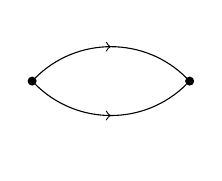
\begin{tikzpicture}
    \path (0,0) node[gdot] (a){} (2,0) node[gdot] (b){};
    \draw[midarrow] (a) to [out=45, in=135] node[above]{} (b);
    \draw[midarrow] (a) to [out=315,in=225] node[below]{$\phantom 5$} (b);
  \end{tikzpicture}
  \hspace{1in}
  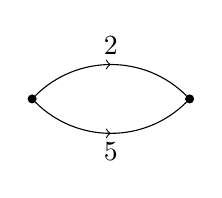
\begin{tikzpicture}
    \path (0,0) node[gdot] (a){} (2,0) node[gdot] (b){};
    \draw[midarrow] (a) to [out=45, in=135] node[above]{$2$} (b);
    \draw[midarrow] (a) to [out=315,in=225] node[below]{$5$} (b);
  \end{tikzpicture}
  \caption{A directed graph with and without weights.}
  \label{fig:path-finding}
\end{figure}
Intuitively these weights are often simple $\Z$ integers.

\subsection{Flows}

Moving on we introduce \emph{flow} values to edges; similar
values to weights, but living not within $\Z$ but instead within an Abelian
group $\Z_n=\sfrac\Z n$.
%(There may also be optimal path algorithms associated
%with flow values, similar to weights on directed edges, but for this paper our
%focus is elsewhere.)
\begin{definition}[$\Z_n$-flow]
  A \emph{$\Z_n$-flow} is a map $f:E\to\Z_n$ which to each $e$ edge of $E$
  assigns a flow ${f(e)\in\Z_n}$ such that there is ``conservation of flow'' at
  every $v\in V$ vertex, by which me mean the sum of the flows into a vertex $v$
  is equivalent to the sum of the flows out it:
  \[
    \sum_{\stackrel e \to v}f(e)=\sum_{v\stackrel e \to}f(e).
  \]
\end{definition}
(And it's important to note equivalence here since $\sum f(e)\in\Z_n$.)
These functions and more specifically counting them will be the ultimate
purpose of this paper.
\begin{definition}[$f$ support]
  The \emph{support} of $f$, denoted $\sgsupp(f)$, is the subset of edges $e$
  whose flows are non-zero:
  \[
    \sgsupp(f)=\{e\in E:f(e)\ne 0\}\subseteq E
  \] 
\end{definition}
If $\sgsupp(f)=E$ (all $e$ edges have $f(e)\ne0$), then $f$ is considered
``nowhere-zero''. For the rest of this report we'll be concerned with these
nowhere-zero $\Z_n$-flows, in particular with counting how many of them can be
made for any particular graph and Abelian group.
%
Figure~\ref{fig:graph-flows} illustrates two different but satisfactory
$\Z_5$-flows on a graph. Without the context of the Abelian group $Z_5$
these flows wouldn't seem to work, but, since $3+2\equiv 0\bmod 5$,
the top and bottom left vertices both have conservation of flow
equal to zero.
\begin{figure}[ht]
  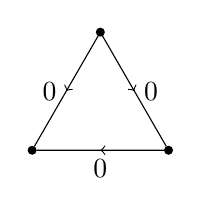
\begin{tikzpicture}
    \path
      (0,1) node (a)[gdot]{}
      ($({cos(  -pi/6 r)},{sin(  -pi/6 r)})$) node (b)[gdot]{}
      ($({cos(-5*pi/6 r)},{sin(-5*pi/6 r)})$) node (c)[gdot]{};
    \draw[midarrow] (a) -- node[right]{0} (b);
    \draw[midarrow] (a) -- node[left]{0} (c);
    \draw[midarrow] (b) -- node[below]{0} (c);
  \end{tikzpicture}
  \hspace{1in}
  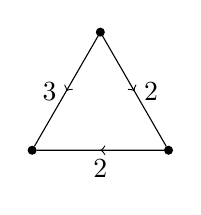
\begin{tikzpicture}
    \path
      (0,1) node (a)[gdot]{}
      ($({cos(  -pi/6 r)},{sin(  -pi/6 r)})$) node (b)[gdot]{}
      ($({cos(-5*pi/6 r)},{sin(-5*pi/6 r)})$) node (c)[gdot]{};
    \draw[midarrow] (a) -- node[right]{2} (b);
    \draw[midarrow] (a) -- node[left]{3} (c);
    \draw[midarrow] (b) -- node[below]{2} (c);
  \end{tikzpicture}
  \caption{An everywhere-zero $\Z_5$-flow and a nowhere-zero $\Z_5$-flow.}
  \label{fig:graph-flows}
\end{figure}

Going forward, $G$ will always refer to a 2-dimensional graph with $V$ vertices
and $E$ edges, $\rho$ to an arbitrary (but fixed) orientation of $G$
and $\Z_n$ to an Abelian group to which $f$ a $\Z_n$-flow maps.
\begin{definition}
  Define a counting function:
  \[
    \varphi_G(n)=\text{the number of $f$ nowhere-zero $\Z_n$-flows on $G$}
  \] 
\end{definition}
As it happens\ldots
\begin{prop}
  The flow-counting function $\varphi_G(n)$ is independent of the orientation
  $\rho$ of $G$.
\end{prop}
(The proof of this is a ``left to the reader'' exercise in the original paper.)
\begin{prop}
  $G$ will not have any nowhere-zero flow if $G$ has a \emph{bridge}---an edge
  whose removal increases the number of connected components of $G$.
\end{prop}

\subsection{Dual graphs}

Consider a graph $G$ as subdividing the plane into connected regions. If two
points lie within a region then they can be connected without intersecting an
edge of $G$. Regions which are neighbors have an edge of $G$ which separate them
(their topological closures sharing a proper 1-dimensional part of their
boundaries).
\begin{definition}[Dual graph]
  The \emph{dual graph} of a graph $G=(V,E)$ is the graph $G^*=(V^*,E^*)$ with
  vertices corresponding to the regions of $G$.
  %
  Two vertices $u^*,v^*\in V^*$
  which correspond to two regions $R_{u^*}$ and $R_{v^*}$ of $G$ are connected via edge $e^*\in
  E^*$ if an original edge $e\in E$ is properly contained within the boundaries
  of $R_{u^*}$ and $R_{v^*}$.
\end{definition}
%Figure~\ref{fig:dual-incomplete} shows a graph with four vertices (solid)
%along with the vertices (hollow) of its dual to demonstrate the regions which
%$G$ subdivides the plane into.
%(However the edges are omitted.
%See Figure~\ref{fig:graphs-and-duals} for complete illustrations of graphs and
%their duals.)
%\begin{figure}[ht]
    %\begin{tikzpicture}
      %\path
        %(0,0) node (a)[gdot]{}
        %(1,0) node (b)[gdot]{}
        %(1,1) node (c)[gdot]{}
        %(0,1) node (d)[gdot]{};
      %\draw (a) -- (b) -- (c) -- (d) -- (a);
      %\path (.5,.5) node[ddot]{} (1.5,.5) node[ddot]{};
  %\end{tikzpicture}
  %\caption{A graph and its (incompletely portrayed) dual graph.}
  %\label{fig:dual-incomplete}
%\end{figure}
In other words there is one $e^*$ for
every edge $e$ that lies between two regions of $G$; it connects the $G^*$
vertices corresponding to the two regions; and it crosses over its
corresponding $e$ edge ($e$ and $e^*$ intersect).
%
But as a single illustration says a thousand words,
Figure~\ref{fig:graphs-and-duals} illustrates a few examples of graphs
(solid dot vertices) and their duals (hollow dot vertices).
\begin{figure}[ht]
  \begin{subfigure}[t]{.3\textwidth}
    \begin{tikzpicture}[
        gdot/.style={draw,shape=circle,fill=black,inner sep=1},
        ddot/.style={draw,shape=circle,fill=white,inner sep=1},
        decoration={markings,mark=at position 0.5 with {\arrow{>}}}
      ]
      \begin{scope}
        %\clip (-2,-1) rectangle (2,2);
        \draw (0,0) node[gdot](a){} -- (1,0) node[gdot](b){};
        \node[ddot](c) at (.5,-.5) {};
        \draw[dedge] (c) to [out=180,in=90,looseness=60] (c);
      \end{scope}
    \end{tikzpicture}
    \caption{Simplest graph with a bridge.}
  \end{subfigure}
  %\begin{subfigure}[t]{.3\textwidth}
    %\begin{tikzpicture}[
        %gdot/.style={draw,shape=circle,fill=black,inner sep=1},
        %ddot/.style={draw,shape=circle,fill=white,inner sep=1},
        %decoration={markings,mark=at position 0.5 with {\arrow{>}}}
      %]
      %\begin{scope}
        %%\clip (-2,-1) rectangle (2,2);
        %\draw (0,0) node[gdot]{} -- (1,0) node[gdot]{} -- ($(1/2,{sqrt(3)/2})$) node [gdot]{} -- cycle;
        %\node[ddot] (a) at ($(1/2,{-sqrt(2)/3})$) {};
        %\node[ddot] (b) at ($(1/2,{sqrt(3)/6})$) {};
        %\draw[dedge] (a) -- (b);
        %\draw[dedge] (a) to [out=180,in=135,looseness=4] (b);
        %\draw[dedge] (a) to [out=0,in=45,looseness=4] (b);
      %\end{scope}
    %\end{tikzpicture}
    %\caption{A complete graph.}
  %\end{subfigure}
  %\begin{subfigure}[t]{.3\textwidth}
    %\begin{tikzpicture}[
      %gdot/.style={draw,shape=circle,fill=black,inner sep=1},
      %ddot/.style={draw,shape=circle,fill=white,inner sep=1},
      %decoration={markings,mark=at position 0.5 with {\arrow{>}}}
    %]
    %\begin{scope}
      %%\clip (-2,-1) rectangle (2,2);
      %\draw (0,0) node[gdot]{} -- (0,1) node[gdot]{};
      %\draw (0,0) node[gdot]{} -- ($({sqrt(3)/2},1/2)$) node[gdot]{} -- (0,1) node[gdot]{} -- ($({-sqrt(3)/2},1/2)$) node[gdot]{} -- cycle;
      %\node[ddot] (a) at (0,-1/2){};
      %\node[ddot] (b) at ($({-sqrt(3)/6},1/2)$){};
      %\node[ddot] (c) at ($({ sqrt(3)/6},1/2)$){};
      %\draw[dedge] (a) to [out=120,in=240] (b);
      %\draw[dedge] (a) to [out=180,in=120,looseness=4] (b);
      %\draw[dedge] (a) to [out=60,in=300] (c);
      %\draw[dedge] (a) to [out=0,in=60,looseness=4] (c);
      %\draw[dedge] (b) -- (c);
    %\end{scope}
    %\end{tikzpicture}
    %\caption{Graph with two connected components.}
  %\end{subfigure}
  \caption{Various graphs and their duals.}
  \label{fig:graphs-and-duals}
\end{figure}

What naturally follows is that if $G$ is a directed graph, we should want
$G^*$ to also be some sort of directed graph.
So, given an orientation of $G$, an orientation on $G^*$ can be induced by
``rotating'' the direction of the edge clockwise. That is, the dual edge $e^*$
will ``point'' east assuming that the primal edge $e$ points north.
%\begin{figure}[ht]
  %\begin{tikzpicture}
    %\draw[->,thick] (.25,0) .. controls (.25,.5) and (.75,.5) .. (.75,1);
    %\draw[->,dedge] (0,.5) -- (1,.5);
  %\end{tikzpicture}
	%\hspace{1in}
  %\begin{tikzpicture}
    %\draw[<-,thick] (.25,0) .. controls (.25,.5) and (.75,.5) .. (.75,1);
    %\draw[<-,dedge] (0,.5) -- (1,.5);
  %\end{tikzpicture}
%\end{figure}


% ------------------------------------------------------------------------------
% 7.6
% ------------------------------------------------------------------------------
\pagebreak
\section{Reciprocity in counting graph flows}

Ultimately the purpose of this report is in providing some intuition into the
following theorem and its proof:
\begin{thm}\label{thm:1.2.5}
  Let $G$ be a bridgeless graph. For every positive integer $n$, the
  reciprocity statement:
  \[
    {(-1)}^{\xi(G)}\varphi_G(-n)
  \]
  counts the number of pairs $(f,p)$,
  where $f$ is a $\Z_n$-flow and $\rho$ is a totally-cyclic reorientation of
  $G/\sgsupp(f)$. In particular, when $n=-1$, the statement equals the
  number of totally-cyclic orientations of $G$.
\end{thm}

Going forward we'll attempt to build some insight into theorem~\ref{thm:1.2.5}
and its proof, and into the propositions upon which the proof relies.

\subsection{Flows and flow spaces}

As a matter of notation, for a vertex $v$, $uv$ is a directed edge pointing
either from a vertex $u$ towards $v$, or from $v$ to $u$. Now to slightly mangle
a previous definition, we now define flows, as opposed to $Z_n$-flows:
\begin{definition}[Flow]
  For $G=(V,E)$ a graph and $\Z_n$ an Abelian group, we define a
  \emph{nowhere-zero flow}, $f:E\to\Z$, to be a map such that $0<f(e)<n$ for all
  $e\in E$, and which for all $v\in V$ with an integer $b_v$ (corresponding to
  $v$) satisfies the equation:
  \[
    \sum_{u\to v}f(uv)-\sum_{v\to u}f(uv)=nb_v.
  \] 
\end{definition}
This should appear very similar to the conservation equation in the
definition of $\Z_n$-flow functions,
but the distinction is that $\Z_n$-flows map to $\Z_n$ and flows map to $\Z$.
Nevertheless, since the difference of the sums in the equation of the definition
above is equal to a multiple of $n$, the sums are indeed congruent modulo $n$,
similar to the conservation in the definition of $\Z_n$-flows.
(I'll present the justification for this distinction between $\Z_n$-flows and
flows soon.)

Next we introduce a specific space of these function
(as well as further mangle the definition of the $f$ flow ``functions''!):
\begin{definition}
  For $\vec b\in\Z^V$ a vector, we define $\calF_G(\vec b)\subseteq\R^E$ to be
  the affine subspace of all $f\in\R^E$ satisfying the equation of the previous
  definition but specifically for $n=1$.
\end{definition}
What I meant by further mangle is that now we don't consider $f$ only as
a function, but now also as a coordinate in $\R^E$ space.
What is $\R^E$ space you ask?
It is ${\lvert E\rvert}$-dimensional, but we don't call it $\Z^{\lvert E\rvert}$
space because: each component of a coordinate is indexed by the edges themselves
as opposed to a more familiar scheme such as $x_1,x_2,x_3,\ldots$.

I certainly had a hard time processing this dual representation, so I'll
attempt to give a brief example to explain this relationship from function to
coordinate:
\begin{example}
  Fix $G$ a directed graph with four edges, $E=\{e_a,e_b,e_c,e_d\}$,
  and $f\in\Z^E$ a nowhere-zero flow on $G$ for some Abelian group $\Z_n$.
  Suppose $f$, being a coordinate in $\Z^E$ space,
  is the coordinate $(4,2,7,5)$ which maps the edges of the graph in the order
  as they appear above.
  Here then is a sort of condensing of $f$'s various representation:
  \[
    f=(4,2,7,5)\in\Z^4,~f(e)\in\{4,2,7,5\}
  \]
	And then the action of mapping:
  \[
    f(e_a)=4,~f(e_b)=2,~f(e_c)=7,~f(e_d)=5
  \]
\end{example}
But what prompts/justifies this mangling of definitions?
Well, what is ultimately being sought after is a way to relate $\Z_n$-flow
functions to lattice points in/on some polytope, and vice versa:
%
flows $f$ which are points in $n{(0,1)}^E\cap \Z^E$.
(Note that $n{(0,1)}^E$ is the n'th dilation of all real-valued points contained
within the ${\lvert E\rvert}$-dimensional open unit cube---no points on the
boundaries. Then the intersection with $\Z^E$ yields only those points that are
lattice/integer point.)

\begin{definition}[Flow space]
  $\calF_G(\vec 0)$ is the \emph{flow space} of $G$ such that each $f$
  satisfies the conservation equation:
  \[
    \sum_{u\to v}f(uv)=\sum_{v\to u}f(uv).
  \] 
\end{definition}
This should now look very familiar to $Z_n$-flows, which from the get-go were
defined with conservation of flow.

(And eventually I get to actually talking about theorem~\ref{thm:1.2.5}!)

%
%
%
\end{document}

